\scanpage{97}
\figure{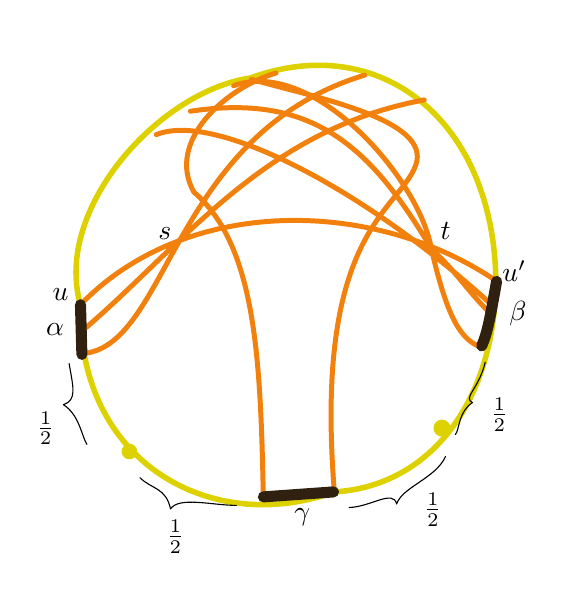
\begin{tikzpicture}[x=.009cm,y=-.009cm,line cap=round,line join=round]
\draw[yellow!70!olive,line width=2pt] (310,450)..controls(271,316)and(420,149)..(550,130)..controls(733,63)and(893,190)..(896,416)..controls(895,584)and(805,706)..(668,714)..controls(493,777)and(305,671)..(310,450);
\draw[orange!80!brown,line width=1.8pt] (310,450)..controls(457,297)and(722,298)..(896,416) (310,489)..controls(455,366)and(568,203)..(795,161) (310,519)..controls(435,514)and(436,209)..(711,126);
\draw[orange!80!brown,line width=1.8pt] (417,210)..controls(500,176)and(714,289)..(889,449) (465,177)..controls(637,151)and(719,226)..(805,371)..controls(839,402)and(855,429)..(886,460) (526,141)..controls(638,100)and(788,272)..(805,371)..controls(828,471)and(847,499)..(875,510);
\draw[orange!80!brown,line width=1.8pt] (586,123)..controls(514,144)and(430,220)..(470,291)..controls(558,367)and(564,528)..(568,723) (551,132)..controls(643,158)and(806,189)..(783,253)..controls(759,318)and(639,346)..(668,712);
\draw[black!75!brown,line width=4pt] (310,450)--(312,520) (897,417)..controls(888,468)and(884,490)..(876,508) (568,721)--(667,714);
\fill[yellow!70!olive] (379,657) circle (11);\fill[yellow!70!olive] (820,624) circle (12);
\draw (294,533)..controls(300,568)and(305,584)..(286,591)..controls(308,605)and(311,633)..(319,647);
\draw (394,694)..controls(410,710)and(431,708)..(437,738)..controls(449,720)and(496,733)..(530,733);
\draw (689,736)..controls(720,735)and(751,710)..(756,731)..controls(764,707)and(811,695)..(825,664);
\draw (881,531)..controls(872,569)and(849,581)..(863,588)..controls(843,601)and(845,625)..(839,633);
\node at (282,435) {$u$};\node at (274,485) {$\alpha$};\node at (429,349) {$s$};\node at (825,346) {$t$};\node at (922,402) {$u'$};\node at (927,463) {$\beta$};\node at (623,750) {$\unsure{\gamma}$};
\node at (261,624) {$\frac12$};\node at (444,777) {$\frac12$};\node at (807,739) {$\frac12$};\node at (901,605) {$\frac12$};
\end{tikzpicture}}
\figure{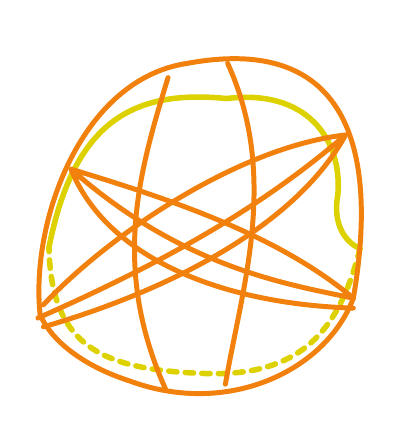
\begin{tikzpicture}[x=.014cm,y=-.014cm,line cap=round,line join=round]
\draw[yellow!70!olive,line width=2pt] (1058,263)..controls(1080,153)and(1130,119)..(1219,128)..controls(1292,119)and(1324,165)..(1320,215)..controls(1315,241)and(1326,258)..(1340,264);
\draw[yellow!70!olive,line width=2pt,dashed] (1340,264)..controls(1320,345)and(1280,382)..(1193,377)..controls(1100,373)and(1060,348)..(1058,263);
\draw[orange!80!brown,line width=1.8pt] (1050,324)..controls(1041,240)and(1087,110)..(1184,96)..controls(1348,66)and(1352,205)..(1334,309)..controls(1309,375)and(1220,417)..(1131,384)..controls(1085,369)and(1059,345)..(1050,324);
\draw[orange!80!brown,line width=1.8pt] (1166,109)..controls(1140,194)and(1114,281)..(1164,392) (1220,96)..controls(1267,199)and(1233,299)..(1218,387);
\draw[orange!80!brown,line width=1.8pt] (1053,315)..controls(1113,251)and(1230,172)..(1327,161) (1048,327)..controls(1177,270)and(1257,221)..(1327,161) (1053,335)..controls(1157,305)and(1279,248)..(1327,161);
\draw[orange!80!brown,line width=1.8pt] (1078,192)..controls(1174,221)and(1267,253)..(1334,309) (1078,192)..controls(1179,281)and(1272,296)..(1334,309) (1078,192)..controls(1110,271)and(1211,314)..(1334,318);
\end{tikzpicture}}
\figure{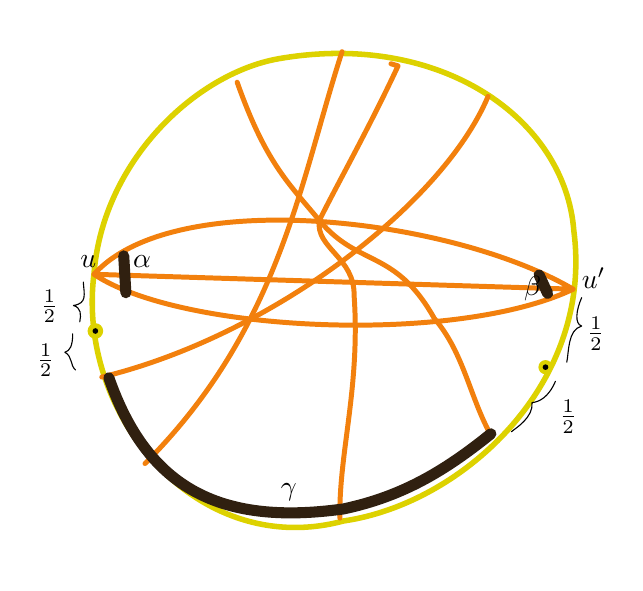
\begin{tikzpicture}[x=.009cm,y=-.009cm,line cap=round,line join=round]
\draw[yellow!70!olive,line width=2pt] (1588,459)..controls(1600,300)and(1731,176)..(1848,155)..controls(2076,115)and(2253,239)..(2265,398)..controls(2293,614)and(2107,783)..(1940,807)..controls(1735,862)and(1563,660)..(1588,459);
\draw[orange!80!brown,line width=1.8pt] (1588,459)..controls(1702,333)and(2092,379)..(2264,480) (1588,459)--(2264,480) (1588,459)..controls(1710,541)and(2098,559)..(2264,480);
\draw[orange!80!brown,line width=1.8pt] (1790,188)..controls(1830,301)and(1862,330)..(1906,383)..controls(1961,449)and(2013,423)..(2068,521)..controls(2110,570)and(2118,632)..(2148,686);
\draw[orange!80!brown,line width=1.8pt] (1938,145)..controls(1879,326)and(1851,535)..(1660,726);
\draw[orange!80!brown,line width=1.8pt] (2007,162)--(2017,165)..controls(1975,255)and(1929,336)..(1906,383)..controls(1900,422)and(1956,435)..(1955,489)..controls(1964,618)and(1933,713)..(1935,803);
\draw[orange!80!brown,line width=1.8pt] (2144,208)..controls(2080,360)and(1838,546)..(1599,604);
\draw[black!75!brown,line width=4pt] (1630,433)--(1633,485) (2216,460)--(2228,486) (1609,605)..controls(1662,756)and(1760,815)..(1940,790)..controls(2020,773)and(2080,739)..(2148,684);
\fill[yellow!70!olive] (1590,539) circle (11);\fill[black] (1590,539) circle (4);\fill[yellow!70!olive] (2225,590) circle (10);\fill[black] (2225,590) circle (4);
\draw (1573,470)..controls(1574,487)and(1579,500)..(1559,503)..controls(1570,506)and(1570,516)..(1568,526);
\draw (1558,543)..controls(1558,560)and(1554,567)..(1547,569)..controls(1558,575)and(1554,587)..(1562,594);
\draw (2276,492)..controls(2268,510)and(2266,529)..(2276,532)..controls(2256,537)and(2258,570)..(2255,583);
\draw (2239,610)..controls(2229,633)and(2216,639)..(2206,640)..controls(2208,661)and(2183,676)..(2177,681);
\node at (1580,441) {$u$};\node at (1656,441) {$\alpha$};\node at (2207,479) {$\unsure{\beta}$};\node at (2293,464) {$u'$};\node at (1863,767) {$\gamma$};
\node at (1525,504) {$\frac12$};\node at (1520,580) {$\frac12$};\node at (2296,543) {$\frac12$};\node at (2257,660) {$\frac12$};
\end{tikzpicture}}

\uline{NB} On suppose qu'il y a au moins une
ps dr qui ne passe pas par $s,t$ i.e.
qu'on n'est pas dans le cas $\mathrm{III}_{pq}$
($p,q\ge1$ — donc pas dans le cas $\unsure{\mathrm{St}_3|\mathfrak R_3}$ non plus)
Quand il n'y a qu'une seule ps. droite
qui ne passe pas $s,t$, \unsure{l'arc} de
spéc. exceptionnel $\unsure{\gamma}$ est de long. $0$.

On suppose qu'il y a une ps. droite
qui ne passe pas $\unsure{u},u'$, i.e. qu'on n'est
pas dans le cas trivial $\mathrm I_m$. Dans
le cas où il n'y en a qu'une,
l'arc de spécialisation \deleted{\unsure{de p.}} exceptionnel—
$\gamma$ est de \uline{longueur} $0$.
\figure{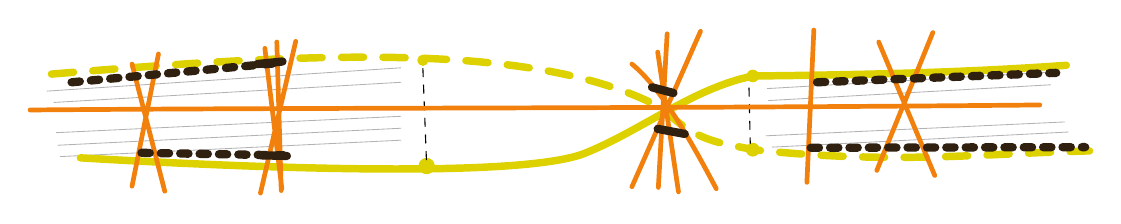
\begin{tikzpicture}[x=.008cm,y=-.008cm,line cap=round,line join=round]
\draw[gray!60,line width=.3pt] (174,1425)--(736,1388) (185,1443)--(736,1411) (189,1491)--(736,1465) (191,1511)--(736,1484) (195,1529)--(736,1503) (1318,1421)--(1767,1395) (1320,1440)--(1768,1415) (1316,1496)--(1790,1474) (1326,1514)--(1796,1490);
\draw[yellow!70!olive,line width=2.7pt,dash pattern=on 8pt off 7pt] (181,1398)..controls(588,1364)and(955,1344)..(1154,1454)..controls(1206,1508)and(1252,1508)..(1295,1518)..controls(1520,1542)and(1660,1524)..(1830,1520);
\draw[yellow!70!olive,line width=2.7pt] (227,1531)..controls(530,1549)and(922,1562)..(1025,1525)..controls(1115,1490)and(1198,1421)..(1295,1401)..controls(1487,1399)and(1640,1395)..(1793,1384);
\fill[yellow!70!olive] (777,1544) circle (13);\fill[yellow!70!olive] (771,1376) circle (9);\fill[yellow!70!olive] (1295,1518) circle (11);\fill[yellow!70!olive] (1295,1401) circle (10);
\draw[dashed] (771,1389)--(777,1544) (1289,1420)--(1291,1508);
\draw[orange!80!brown,line width=1.7pt] (147,1455)..controls(615,1451)and(1130,1453)..(1751,1447);
\draw[orange!80!brown,line width=1.7pt] (309,1382)--(361,1584) (351,1366)--(309,1576) (520,1357)--(547,1580) (539,1347)--(546,1583) (569,1346)--(513,1587) (1103,1382)..controls(1150,1420)and(1200,1510)..(1237,1580) (1144,1363)--(1177,1585) (1159,1334)--(1145,1578) (1212,1330)--(1103,1577) (1392,1328)--(1381,1570) (1495,1347)--(1584,1559) (1581,1332)--(1492,1551);
\draw[black!75!brown,line width=3pt,dash pattern=on 3pt off 4pt] (213,1411)--(535,1381) (324,1523)--(550,1527) (1397,1411)--(1777,1396) (1387,1515)--(1823,1514);
\draw[black!75!brown,line width=3pt] (508,1382)--(548,1378) (514,1527)--(555,1528) (1135,1419)--(1169,1428) (1144,1485)--(1187,1493);
\end{tikzpicture}}
\figure{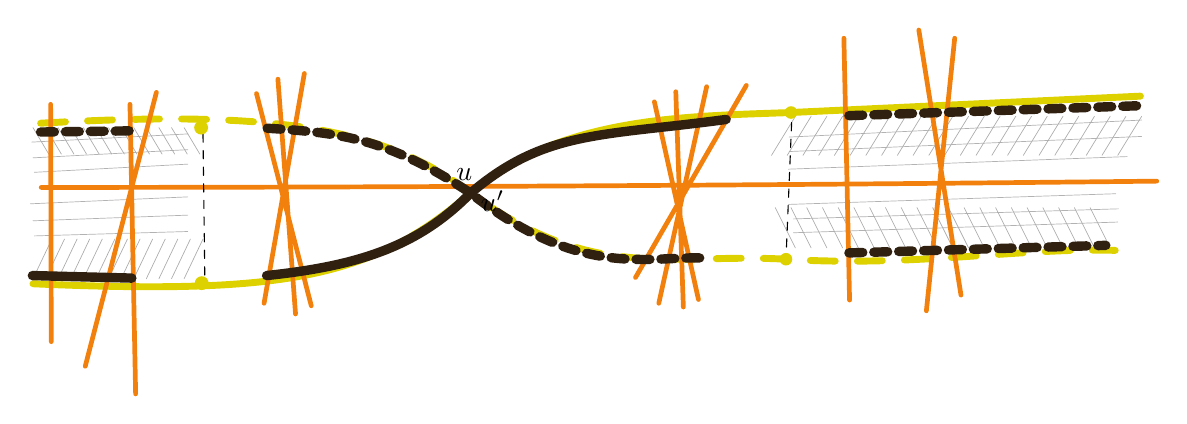
\begin{tikzpicture}[x=.008cm,y=-.008cm,line cap=round,line join=round]
\draw[gray!60,line width=.25pt] (82,1768)--(330,1755) (84,1793)--(330,1780) (86,1816)--(330,1803) (80,1866)--(330,1855) (84,1893)--(330,1884) (86,1917)--(330,1910) (1285,1760)--(1845,1733) (1285,1783)--(1845,1759) (1284,1811)--(1822,1791) (1284,1867)--(1804,1850) (1292,1890)--(1808,1874) (1292,1912)--(1807,1895);
\foreach \x in {84,104,...,324}\draw[gray!65,line width=.25pt] (\x,1745)--++(25,42);
\foreach \x in {84,104,...,324}\draw[gray!65,line width=.25pt] (\x,1985)--++(30,-63);
\foreach \x in {1295,1320,...,1845}\draw[gray!65,line width=.25pt] (\x,1727)--++(-38,62);
\foreach \x in {1295,1320,...,1800}\draw[gray!65,line width=.25pt] (\x,1936)--++(-32,-64);
\draw[yellow!70!olive,line width=2.5pt,dash pattern=on 9pt off 8pt] (96,1738)..controls(430,1719)and(634,1735)..(779,1849)..controls(974,1992)and(1095,1944)..(1280,1954)..controls(1480,1967)and(1660,1935)..(1803,1940);
\draw[yellow!70!olive,line width=2.5pt] (84,1993)..controls(494,2011)and(625,1981)..(779,1849)..controls(918,1727)and(1123,1727)..(1288,1721)--(1843,1695);
\draw[orange!80!brown,line width=1.7pt] (97,1840)..controls(605,1840)and(1230,1837)..(1869,1830);
\draw[orange!80!brown,line width=1.7pt] (112,1708)--(113,2085) (238,1708)--(247,2168) (280,1689)--(167,2124) (439,1691)--(526,2028) (473,1668)--(501,2041) (515,1659)--(451,2024) (1071,1704)--(1141,2018) (1105,1688)--(1117,2030) (1154,1680)--(1078,2024) (1217,1678)--(1041,1983) (1372,1603)--(1381,2019) (1491,1590)--(1558,2011) (1548,1603)--(1503,2036);
\draw[black!75!brown,line width=3.4pt,dash pattern=on 5pt off 4pt] (96,1752)--(249,1750) (456,1746)..controls(575,1753)and(649,1763)..(779,1849)..controls(951,1984)and(1057,1950)..(1143,1952) (1380,1726)--(1847,1710) (1380,1944)--(1788,1932);
\draw[black!75!brown,line width=3.4pt] (83,1980)--(241,1984) (455,1980)..controls(596,1965)and(694,1936)..(779,1849)..controls(897,1749)and(985,1759)..(1185,1732);
\draw[dashed] (354,1755)--(357,1991) (1289,1737)--(1280,1954);
\fill[yellow!70!olive] (351,1745) circle (11);\fill[yellow!70!olive] (352,1992) circle (11);\fill[yellow!70!olive] (1288,1721) circle (10);\fill[yellow!70!olive] (1280,1954) circle (10);
\node at (769,1820) {$u$};\node at (814,1862) {$u'$};
\end{tikzpicture}}
\margin{96}
